% THIS IS SIGPROC-SP.TEX - VERSION 3.1
% WORKS WITH V3.2SP OF ACM_PROC_ARTICLE-SP.CLS
% APRIL 2009
%
% It is an example file showing how to use the 'acm_proc_article-sp.cls' V3.2SP
% LaTeX2e document class file for Conference Proceedings submissions.
% ----------------------------------------------------------------------------------------------------------------
% This .tex file (and associated .cls V3.2SP) *DOES NOT* produce:
% 1) The Permission Statement
% 2) The Conference (location) Info information
% 3) The Copyright Line with ACM data
% 4) Page numbering
% ---------------------------------------------------------------------------------------------------------------
% It is an example which *does* use the .bib file (from which the .bbl file
% is produced).
% REMEMBER HOWEVER: After having produced the .bbl file,
% and prior to final submission,
% you need to 'insert' your .bbl file into your source .tex file so as to provide
% ONE 'self-contained' source file.
%
% Questions regarding SIGS should be sent to
% Adrienne Griscti ---> griscti@acm.org
%
% Questions/suggestions regarding the guidelines, .tex and .cls files, etc. to
% Gerald Murray ---> murray@hq.acm.org
%
% For tracking purposes - this is V3.1SP - APRIL 2009

\documentclass{acm_proc_article-sp}

\usepackage{soul}

\begin{document}

\title{Games for Computational Thinking}
% \subtitle{[Extended Abstract]}
%
% You need the command \numberofauthors to handle the 'placement
% and alignment' of the authors beneath the title.
%
% For aesthetic reasons, we recommend 'three authors at a time'
% i.e. three 'name/affiliation blocks' be placed beneath the title.
%
% NOTE: You are NOT restricted in how many 'rows' of
% "name/affiliations" may appear. We just ask that you restrict
% the number of 'columns' to three.
%
% Because of the available 'opening page real-estate'
% we ask you to refrain from putting more than six authors
% (two rows with three columns) beneath the article title.
% More than six makes the first-page appear very cluttered indeed.
%
% Use the \alignauthor commands to handle the names
% and affiliations for an 'aesthetic maximum' of six authors.
% Add names, affiliations, addresses for
% the seventh etc. author(s) as the argument for the
% \additionalauthors command.
% These 'additional authors' will be output/set for you
% without further effort on your part as the last section in
% the body of your article BEFORE References or any Appendices.

\numberofauthors{3} % in this sample file, there are a *total*
% of EIGHT authors. SIX appear on the 'first-page' (for formatting
% reasons) and the remaining two appear in the \additionalauthors section.
%
\author{
% You can go ahead and credit any number of authors here,
% e.g. one 'row of three' or two rows (consisting of one row of three
% and a second row of one, two or three).
%
% The command \alignauthor (no curly braces needed) should
% precede each author name, affiliation/snail-mail address and
% e-mail address. Additionally, tag each line of
% affiliation/address with \affaddr, and tag the
% e-mail address with \email.
%
% 1st. author
\alignauthor
Panagiotis Apostolellis\\
 \affaddr{Virginia Tech}\\
 \affaddr{2202 Kraft Dr}\\
 \affaddr{Blacksburg, VA, 24060}\\
 \email{panaga@vt.edu}
% 2nd. author
\alignauthor
Chris Frisina\\
 \affaddr{Virginia Tech}\\
 \affaddr{2202 Kraft Dr}\\
 \affaddr{Blacksburg, VA, 24060}\\
 \email{special@vt.edu}
% 3rd. author
\alignauthor
Michael Stewart\\
 \affaddr{Virginia Tech}\\
 \affaddr{2202 Kraft Dr}\\
 \affaddr{Blacksburg, VA, 24060}\\
 \email{tgm@vt.edu}
}
\date{12 January 2014}
% Just remember to make sure that the TOTAL number of authors
% is the number that will appear on the first page PLUS the
% number that will appear in the \additionalauthors section.

\maketitle
\begin{abstract}
Computational Thinking (CT) is present in every domain just as the other core literacy skills of reading, writing, and arithmetic. Unfortunately, current curriculum both introduces and teaches CT concepts predominantly in programming courses. We designed two physical CT games and had the opportunity to informally test and observe one of them in action. Our vision is to have K-12 students engage in different games that introduce and broaden their understanding of CT throughout their education. The development cost for each age-appropriate game is minimal, increasing feasibility of implementation and target audience participation. Individually, the games challenge students to grow their understanding of CT in an acute, focused activity, while collectively they maintain CT as a core literacy skill throughout students' education.
\end{abstract}

% A category with the (minimum) three required fields
\category{H.4}{Information Systems Applications}{Miscellaneous}
%A category including the fourth, optional field follows...
\category{D.2.8}{Software Engineering}{Metrics}[complexity measures, performance measures]

\terms{Theory}

\keywords{ACM proceedings, \LaTeX, text tagging} % NOT required for Proceedings

\section{Introduction}
Since Wing's influential work preceding\cite{wing2006computational} and during\cite{wing2008computational} her service to the National Science Foundation, the research around Computational Thinking (CT) has exploded into myriad lines of divergent pursuits. Following prior work such as the Great Principles of Computing\cite{denning2003great} on the topic of defining either prerequisites for computer science or its transferable skills, and coinciding with other work attempting to broaden participation in computer science (e.g. CS Principles\cite{csprinciples}), Wing et al. have demonstrated the immensity of the research space around CT. Much of this work has offered working definitions of CT\cite{allan2010computational,barr2011bringing,national2010report}, but none has become the standard.

Despite the current diversity of views, various institutions have committed to agendas supportive of ``computational thinking.'' In their recently adopted Long Range Plan, Virginia Tech (VT) identifies CT as a fundamental competency of a broad general education \cite{vtlongrange}. In support of this mission, Dr. Dennis Kafura developed a graduate course to ``develop a better understanding of what CT means at the university level of teaching and learning, and how CT could be made accessible to students in all disciplines at VT.''

In pursuit of this understanding, our group developed activities to be performed with students at a younger age, prior to their entrance in college, to help them develop CT.


\section{Computational Thinking}
The research around CT is divergent in its definition. This is in part due to the variety of research agendas that are served by work on CT. While certainly different research agendas might simultaneously be served by a single pursuit, this at least introduces tensions. 

Our working definition is as follows:

Computational Thinking (CT) involves using cognitive skills to represent abstracted modeling, construct and evaluate processes, and apply appropriate strategies to enable us to interact in structured and creative problem-solving techniques to address problems and assumptions. Additionally, a computational thinker reflects on how we are affected by the computational artifacts with which we (must) interact.

\subsection{Recruitment of Computer Scientists}
Each year, for several years now, there have been insufficient computer scientists for market demand. The result is increased reliance on imported laborers, exported labor, and decreased productivity, innovation, and security. To this end, some believe that supporting an agenda of teaching CT to many if not all students could increase the number of computer scientists.

\subsubsection{Broadening Participation}
If indeed, ``Computer science is no more about computers than astronomy is about telescopes,''\cite{cs-astronomy} why do so many ``CS0'' courses begin with computers, and usually with programming? Especially as they were historically taught (with some notable exceptions such as Papert et al.)\cite{logo-readings}, programming and its allure through precise control over the machine does not appeal to all.

In order to broaden the participation in computer science to more diverse demographics of students, it may be necessary to change the entry routes and introductions to be similarly diverse. In this vein, projects like ALICE\cite{pausch1995alice}, Media Computation\cite{guzdial2003media}, and CS Unplugged\cite{csunplugged} are useful exemplars. Many of the definitions developed for CT have specifically excluded programming; however many of these same works then attempted to teach CT using some form of programming.

Activities that differ from programming may appeal to different demographics. Additionally, some demographics that may lack resources (human, electronic, and monetary) sufficient for learning programming may be able to utilize CS Unplugged or CT curricula.

\subsubsection{Increasing Participation}
Aside from efforts attempting to broaden participation, there are efforts that merely seek to increase participation. How should someone know they might be interested in computer science? From the earliest education, we expose students to reading, writing, and arithmetic. When are they exposed to computer science? Unfortunately, only after a student [or their parent(s)] elects to take a programming course do they encounter computer science. 

CT, rather than programming, might be taught explicitly, as its own subject, or implicitly in the context of other subjects, at ages much younger than a high school programming course. Then, more students will have an opportunity to recognize an affinity for skills that would support a pursuit of education in computer science, or at minimum, understand the benefits of applying CT in fields of their own interest.

\subsection{Preparing the 21st Century Citizen}
While improving recruitment of computer scientists is a major focus of many CT research agendas, an emerging concern is the general public's preparedness for the increasingly technological modern age. Many researchers' definitions of CT attempt to specify important skills related to technology and computation that the researchers themselves predict to be necessary as our society continues to adopt technological solutions in virtually every domain. Some call this computational or technological literacy rather than CT, but as Professor Dane Webster mentioned in a presentation to our class, ``Doesn{'}t teaching math students to use a pencil help them to think mathematically?''

\subsubsection{Caveats}
While our group (like many of the researchers before us) consider abstraction to be a critical part of CT, we believe that it is necessary to simultaneously teach the dangers of abstraction. In line with Blackwell, et al., we agree that abstraction might be ``antagonistic to reasonable human concerns'' \cite{blackwell2008abstract}. Along the same lines, Turkle and Papert have argued long ago that ``concrete and personal approaches'' to computing should not be downplayed in favor of formal and ``abstract approaches'', nor should they be dismissed as more inferior \cite{turkle1990epistemological}. Their thesis, based on ethnographic and psychology investigations, aligns well with the theory of situated learning which postulates that people learn contextually, by being actively engaged in authentic (learning) activities, and not in the decontextualized and abstract manner of formal education \cite{brown1989situated}.

\subsection{Educational and Computational Thinking Games}
The tradition of using games for education is a long one. Children grow up and get to know the world around them through play. Most of their interactions in an early age are through touch, and other senses as well, and this is why most of the games of early childhood are tangible. This realization was what led the German educator Friedrich Froebel to build a series of wooden blocks known as Froebelgrabe (i.e., Froebel gifts) in an attempt to foster children's self-directed activity in exploring the world and using the environment as a learning aid \cite{liebschner1992child}. Based on this notion of learning by doing, researchers at MIT Media Laboratory have coined the term objects-to-think-with as a means to leverage the power of computation in the exploration process \cite{resnick1998digital,schweikardt2006roblocks}. LEGO/Logo is maybe the most famous offspring of this approach where students are learning to program by controlling enhanced LEGO structures (equipped with motors and sensors). Resnick et al. has proposed ``digital manipulatives'' as a continuation of this work where students are called to control through Logo programming other tangible artifacts like blocks, balls, beads, and badges \cite{liebschner1992child}.

Other researchers have also argued about the educational benefit of using computationally-enhanced construction kits where kids build 3D models and ``learn through tactile experiences'' \cite{eisenberg2002computationally}. Such smart artifacts are equipped with technology that allows them to communicate with each other, with computers, and eventually provide feedback about their state to their users. Various systems have been proposed since then, employing a variety of advanced technologies like programming robotic motion of motorized pieces through kinetic memory \cite{raffle2004topobo} or creating structures with blocks embedding sensors, logic circuits, and actuators for science education \cite{schweikardt2006roblocks}. Although these are exceptional examples of high-tech application in the service of informal education, they are mainly research projects that in most cases do not become commercialized. On the contrary, we were interested to investigate how low-cost games with easy to manufacture components can be leveraged to provide CT exposure to very young children. 

For such an audience, motivation is believed to play a significant part in the learning process; this is even more the case if learning objectives are intrinsic to the goal of the game \cite{malone1987making}. To motivate them, learners are immersed in a fantasy world and are asked to do challenging tasks by instigating their curiosity. These practices have been used in many educational games, including ones that teach about computer science and programming. Examples include either stand-alone games that leverage elements of fun to teach simple programming concepts like pattern recognition and recursion (e.g., Light-Bot), but also tools that leverage the students innate creativity to learn programming through game building (e.g., Scratch, Snap, and AgentSheets).

It is natural to want to extend the enthusiasm and promise of educational games to every domain, CT should be no exception. To offer an environment in which play and hopefully fun also result in learning CT would be ideal. However unlike many other domains, the definition and scope of CT is still in flux, making it challenging to argue (or at least to have agreement) that a given activity would support CT, without being so attached to computers and CS concepts. For example, Berland and Lee explored the CT that might be taught in an existing, commercialized board game: Pandemic \cite{berland2011collaborative}. As Pandemic is essentially a graph-theoretical representation of several major cities in the world, and the game is cooperative, with the result that the game mechanic is the opponent rather than the other human players, there is some promise to this idea. The aspects of CT they chose to focus on were conditional logic, distributed processing, debugging, simulation, and algorithm building. 

During our research for other popular games that can potentially be used for teaching CT indirectly although they have not been designed for this purpose, we reviewed many current, commercialized games, but also came up with some hybrid ideas (see Appendix: Computational Thinking in Existing and Imagined Games). And, to our delight, exactly contemporary with this stage of our work, CT was getting attention from a much broader audience through a Kickstarter project, teaching programming to little kids using a board game \cite{robotturtles}. Having completed this extensive analysis, and been unsatisfied, and also questioning whether it would be possible to teach CT in tangible games, we decided to construct our own low-cost games.

\subsubsection{RabBit EscApe}
Besides the identified need to involve children with CT from an early age, few endeavors focus on primary school children and younger. RabBit EscApe is a board game with tangible wooden pieces intended for ages 8 and up. As shown from previous work, tangible wooden blocks like the Froebel blocks\cite{liebschner1992child} are very engaging and educational for this age group, contributing to children's emotional, social, and physical development through play. The game was inspired by the combination of the magnetic tile game Picasso-Tiles\cite{picassotiles3d} and the work from Weller et al. on objects-to-think-computationally-with using the Posey construction kit and a pacman-style game to teach state machine representations to children \cite{weller2008escape}. In our approach we decided to avoid using any electronic medium like a computer in an attempt to reach younger ages which are accustomed to fiddling with tangible objects but are not yet ready to make connections between physical objects and virtual representations. The outcome was a combination of a board game with wooden pieces with encased magnets, described in the following section.

\subsubsection{Design}
Our idea started by using manipulatives that have been a favorite kids' educational toy for a long time, but also wanted to provide some structure to the game to better support CT, hence we decided to construct a board, as well. We opted for wooden pieces both for their elegance and warm feeling, but also for health reasons preferred over plastic or other chemically manufactured materials. 

The game is comprised of fourteen different shapes of wooden pieces half an inch thick which we call bits; each bit is equipped with small magnets (1/16'' thick and a diameter of 1/4'') which are encased in different sides of the bit and can attract or repel each other depending on polarity. By putting two bits together, you can make a block which is usually a square, rectangle, or hexagon. Other weird shapes can be constructed as well for more advanced levels. Magnets are placed either at the middle of a bit's side or near one of the side's corners to allow a variety of path formations. From the fourteen different shapes, there are twenty-nine unique bits due to varying magnet placement and polarity combinations. We also provide a selection of boards with a path comprised of all, or a subset, of these 29 bits. Boards are of different levels of difficulty depending on the combination of pieces and the ambiguity in block formations.

The goal of the game is to put the bits on the predefined path and help the rabbit (another piece) escape from the fierce apes; hence the name of the game RabBit EscApe! The apes are square pieces which are placed in different positions on the board and the player(s) need to make sure that the adjacent bit repels an ape piece (i.e., same polarity magnets), instead of attracting it which is the objective when constructing the path. Figure 1a below depicts the path of LevelA as it was designed on the computer, and Figure 1b is a photograph of the actual board with most pieces placed in the right order (two are left intentionally off the path for illustrative purposes).
\begin{figure}
  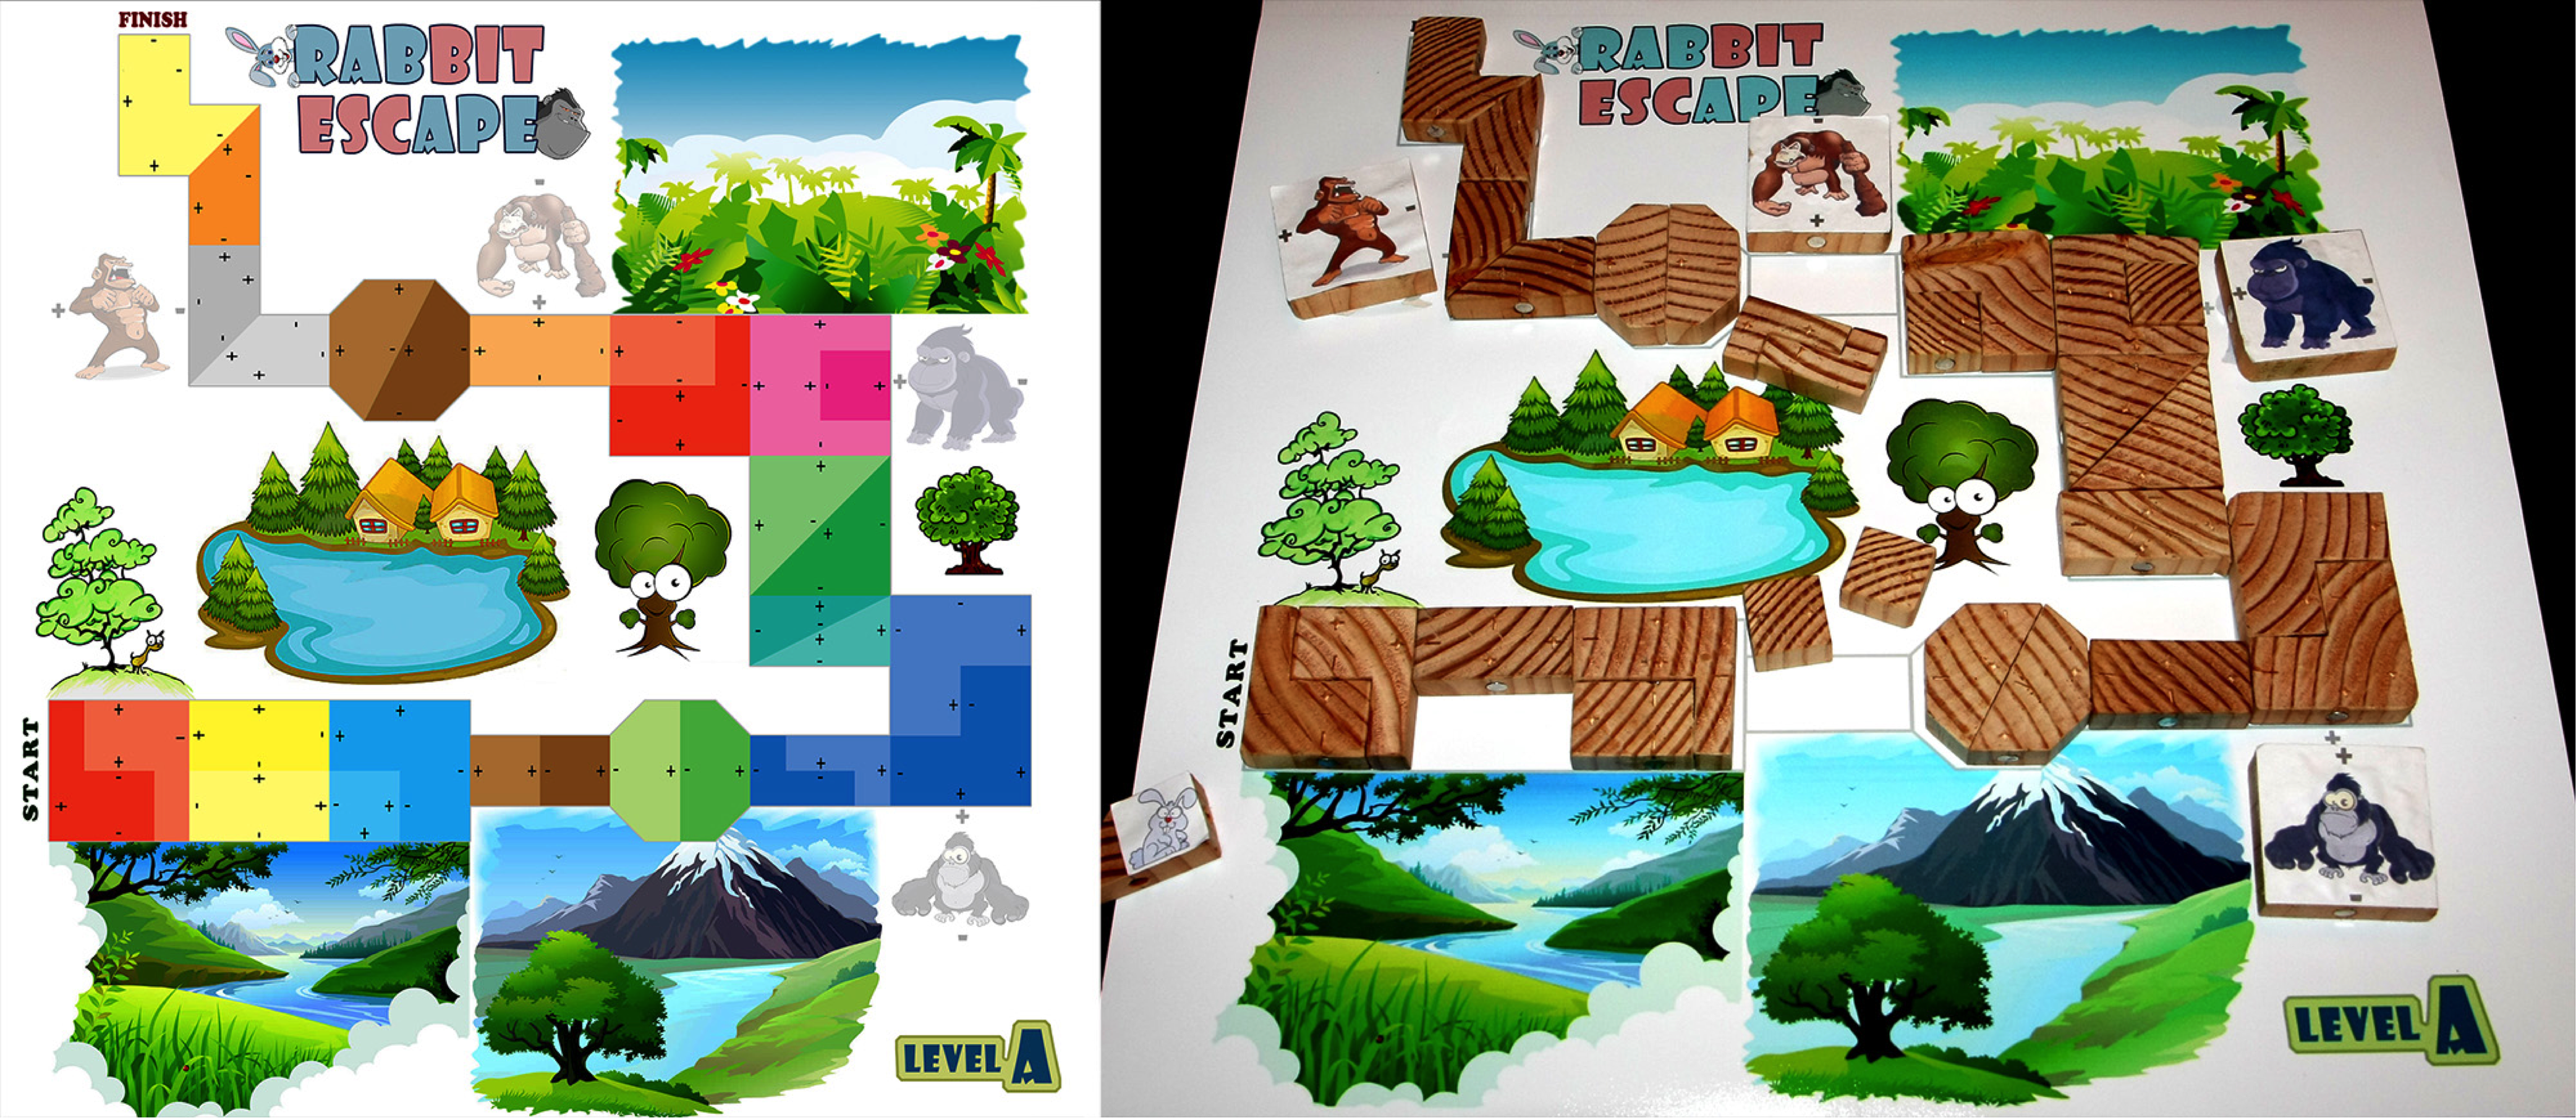
\includegraphics[width=0.48\textwidth]{boardgame.png}
  \caption{ (a) Designed completed board for Level A; (b) Physical game of the same board with most bits in place. }
  \label{fig:board-game}
\end{figure}

What makes the game especially challenging is the correct identification of the bits' properties and subsequent utilization of these properties to construct the blocks and then the whole path. These properties are:
\begin{itemize}
  \item{the size of each bit}
  \item{the position of the magnet on the bit}
  \item{the polarity of each magnet (engraved on the bit's long side)}
  \item{the orientation of the bit (or whole block)}
\end{itemize}

Players must combine all these attributes in order to put the bits next to each other in such a manner that they stick together at the right place (center or top of the bit's side), while also repelling the enemies positioned around the board. The one level we designed for this course utilized all 29 pieces and all 4 enemies; we have made two variations of it, one with the block divisions drawn on the map and a more difficult one without them. Both of them were test during an informal evaluation we ran in a school near VT, described in the section: Evaluation and Observations.

\subsubsection{Play Strategies}
Training - Scaffolding
In order to help players understand the game mechanics and the importance of the different piece properties and how they affect completing the board effectively, we suggest a training session preceding the actual gameplay. The session's purpose is to scaffold the players' understanding of how putting the pieces together allows them to construct different shapes and satisfy the activity objective. This need derived from our informal evaluation in a primary school and is described in the following section.

Scaffolding includes levels of increasing difficulty, starting from making a single block (comprised of two bits) and moving on to more complicated shapes. At some points they will have the option to construct the different shapes using more than one combination of bits, and will have to take into account other piece properties and examine the implications of their choices. This mental modeling of the different affordances of each piece and the possible blocks it can construct will enable them to be more efficient in the actual activities, without demanding extra cognitive load to process them during gameplay. 

Another idea to aid the bit selection and usage process is to have a separate ``cheat sheet'' with all pieces and their amount, next to the actual game boards. Players can cross out any pieces that have been used with a marker in order to keep track of what has been used and what is still available. This cheat sheet can be used during the initial sessions where players are learning the available bits and practicing with the strategies of putting them together. Then, these mental aids can be progressively removed, letting the users depend on their ability to recognize the physical pieces. This is a common process of scaffolding in instructional design, also called fading, because the additional information (scaffold) is removed (faded) over time \cite{driscoll2005psychology}.

The possible suggested activities for teaching CT with the game are described in more detail in the section that follows, although we understand that there are many variations that can derive from the suggested ones.

\subsubsection{Individual or Collaborative}
Players are given a predefined number of bits and a board and need to complete the board with all the pieces (i.e. build the path printed on the board), in a predefined amount of time (optional). They are playing individually or as a team and can either place a block on the board in turns or negotiate about path building. This is the mode we have used during the school assessment, described below. To increase difficulty they can add one or more of the enemy blocks by rolling the dice to decide enemy position; polarity is predefined on each board but players can reverse it to make the game easier or more difficult (preferably before starting the placement of the blocks).

Since each player has to conduct a rule-based plan based on their understanding of the game and combine their shared knowledge we consider this to be a manifestation of distributed computation. Through the ``considerations, contingencies, and strategy formation'' of multiple parties a distributed cognition of different knowledge resources is created<CITATION NEEDED>\cite{} and has to be maintained during the game to reach completion. Distributed computation thinking was indicated as one of the distinguishing properties of CT compared to computer science, according to the National Research Council \cite{national2010report}.

\subsubsection{Competitive}
Players are playing against each other and have to complete the path but starting from different directions. They roll the dice and can place as many bits as the number rolled. This mode demands very good planning, since making the wrong choice will render the board impossible to complete. Players get 1 point for every correct bit placed. They can change bits or blocks by deducting double the points of bits (e.g., 4 points for taking out 2 bits = 1 block). Taking off bits of the opponent's path is forbidden unless she consents, in which case they both lose the exact number of points as the bits (e.g., 2 points each for taking out 2 bits).

The competitive mode demands efficient modeling skills since opponents would need to simulate the construction a large portion of the board with the available pieces, to avoid the cost of losing points and negotiating retraction of a previous block or bit placement. In a sense the effective combination of bit properties can be thought as algorithms that players need to compile during simulation in order to avoid these adverse consequences. For example, deciding which two bits need to be placed together in a way to accommodate locking the blocks with adjacent ones (i.e., having the magnets in the right position and polarity), and do this for a series of blocks is a complex cognitive process similar to compiling an algorithm and testing hypothesis (simulation). Both model building and simulation (forming and contrasting hypotheses) have been defined as foundational aspects of CT and revealed increased benefits compared to traditional methods of instruction \cite{wilensky2006thinking}.

\subsubsection{Board Construction}
Players can use all the bits or a random subset and make a custom path on an empty board. They have to do this by drawing the blocks on the board but without placing the bits. They will need to use the bits and blocks by creating a mental model of the path, taking each ``used'' block out before moving on, until they believe they have drawn the whole path. The only requirement would be to start the path from an entry point on one side of the board and finish on an exit point at another side. Adding enemies would be optional to increase the difficulty of the game. The second player, or another group of players, can then use this custom board to play the game in either of the first two ways.

Like the previous activity, this one demands very good planning and ability to combine bit properties in order to make a playable board. Considering bits and their properties to be the data, players need to construct sets of pieces as part of the path using conditional logic during the process similarly to writing an algorithm (e.g., if I place this bit here, then this block has a minus on the bottom and needs a big square piece with a plus on the top center). This activity in particular demands the complex skill of combining different requirements to build a set of steps that will lead to an efficient solution to a problem (i.e., build a path from point A to point B, using X number of pieces, and avoid Y enemies) and has been defined as procedural thinking - teaching concept abstraction into algorithms\cite{papert1980mindstorms}, a core concept of CT\cite{national2010report}.

\subsubsection{Development of CT}
RabBit EscApe satisfies most of the characteristics of the Operational Definition of CT for K–12 Education as defined by the International Society for Technology in Education (ISTE)\cite{operationalct}. More specifically, students playing the game should be able to: 1) logically organize and analyze data, 2) automate solutions through algorithmic thinking (a series of ordered steps), and 3) identify, analyze, and implement possible solutions with the goal of achieving the most efficient and effective combination of steps and resources. Considering the game mechanics and suggested activities discussed previously, we can make the following arguments considering support of these three characteristics:

\begin{enumerate}
\item{Bits have to be organized in blocks and block combinations that are meaningful according to bit properties and the printed path's form; pattern recognition is important in this process for identifying which bits create blocks that can fit the path printed on the board while also attracting adjacent blocks or repelling enemy blocks (demands analyzing the board based on possible bits combinations and organizing them on the path)}
\item{Game setup C demands that players devise some kind of strategy for correctly utilizing bits and matching the polarity and magnet position; for this purpose they need to come up with some kind of ``recipe'' for putting bits together while drawing the path on the board, also accounting for the remaining pieces (demands some kind of procedural or algorithmic thinking)}
\item{In all game setups, especially A and B, players need to correctly identify the combination of blocks and bits by analyzing the path's comprising shapes and then simulate possible solutions for effectively completing the board, with the least number of bits and in the minimum time (efficiency).}
\end{enumerate}

Additionally, the game supports all dispositions and attitudes that are essential dimensions of CT, as expressed by the aforementioned definition which is pertinent to K-12 students:
\begin{itemize}
       \item Confidence in dealing with complexity
       \item Persistence in working with difficult problems
       \item Tolerance for ambiguity
       \item The ability to deal with open-ended problems
       \item The ability to communicate and work with others to achieve a common goal or solution
\end{itemize}

\section{Evaluation and Observations}
We did not have sufficient time to complete a rigorous evaluation of RabBit EscApe. However we did run an informal pilot. As much as possible without violating observation protocols of the children's school and our own institution, we followed Brandt's anecdote and interrogator method \cite{brandt1972studying}. In order to protect our subjects' privacy, we took no notes during the actual session, but immediately thereafter wrote up the observations, and later in the same day, we interrogated each other's accounts. Our notes, including revisions from interrogation, are included in the Appendix (Informal Observation Interrogation-Augmented Anecdotes).

From our pilot, we learned how much this activity must be pedagogically scaffolded. Prior to attempting a full puzzle, we should familiarize the participants with the pieces by providing simple puzzles involving very few (2-4) pieces. Then, we would gradually increase the difficulty by giving similar, but subtly different pieces. By scaffolding the activity in such a way, the students would approach the challenging problem shown in Figure 1 with an understanding of the properties of the pieces as described above (this process is described in more detail under the first section of the Play Strategies).

Among many other interesting observations, one that we thought supported this scaffolded introduction, as well as the potential for RabBit EscApe to promote CT is captured in Michael's notes. Regarding the students' process for searching, Michael noticed the students describing to each other the shapes they wanted for a particular position on the board. At first the students described only the shape of the piece; however, they soon learned that the piece placement was too tightly constrained to merely try to swap out pieces of the same shape. After all, they could not be sure whether it was the piece in question that needed to be replaced, or its surroundings. They then realized that they should specify the shape and also the polarities of the magnets; however, even this was an underspecification. Because similarly shaped pieces may have the same number of magnets, but in different positions within a piece, they had to also specify the magnet locations. Through a sort of discovery process, the students used incremental formalism\cite{shipman1999formality} to indicate what pieces they were looking for, and simultaneously to enhance their spoken representation of the pieces (and likely their mental models of them as well).

Additionally, Chris and Panagiotis, supervising another group, were very effective in leading students to evaluate the different properties of a missing piece. Questions like ``What does this big piece need to have?'' and ``What do we know about it?'' by pointing on the larger block on the board (at the bottom right of Figure 1b) prompted students to use conditional logic in identifying the properties and eventually the piece. More specifically, one of the students started to respond to these prompts by saying ``It is a big piece'' and then ``it needs to have a plus magnet here'', while pointing at the bottom where the ape is, and ``it should have two more magnets on these sides'', pointing at the top and bottom left where the large piece connects with the remaining path. Such instances were indications that students could grasp the conditions that need to be in place in order for the pieces to be placed successfully.

\subsection{Discussion}
Fabricating our own game was an interesting challenge. For future work, we might propose just such an exercise for high school or later students in a ``shop''-style class. The records to keep track of which pieces have been cut, tapped, sanded, and implanted with magnets is a challenge in itself, but to have consistent results at the end, the use of various custom jigs is important. To determine the kind of physical and process scaffolding needed to produce consistent sizes of pieces in a timely fashion is important and difficult. 
From RabBit EscApe's theoretical design, and our informal observations, we believe it shows promise for teaching CT. In the Development of CT section above, we outline the various elements of CT that RabBit EscApe was designed to influence. Then in our Observation section, we detail observations that support our implementation's successful realization of these design intentions. 

\section{Conclusions}
As CT continues to be discussed in academic and professional communities and until a more concrete definition emerges, a significant leap must be made to educate our communities' youth as society continues to develop systems with which they must interact, whether or not they can understand them. 

VT has embarked on a bold course to develop the CT capabilities of all its graduates. Simultaneously the US National Science Foundation is funding research into how to develop these skills in the broader population. While we think that VT can be effective in this pursuit, we believe that to truly change the CT of the population as a whole, we must have myriad interventions at various stages of an individual's formal and informal education.

In support of education students at a younger age (than undergraduate students), we have developed two proofs of concept for how it might be possible to teach CT in a relatively explicit way. We believe that addressing CT directly, in conjunction with more subtle interactions such as integrating CT with core content in existing formal education curricula (Tatar, et al.) will best facilitate the learning of CT and its successful transfer and application to each individual's area of interest or expertise.


%\end{document} % This is where a 'short' article might terminate

%ACKNOWLEDGMENTS are optional
\section{Acknowledgments}
Dane Webster, our CT class?

%
% The following two commands are all you need in the
% initial runs of your .tex file to
% produce the bibliography for the citations in your paper.
\bibliographystyle{abbrv}
% \bibliography{sigproc} % sigproc.bib is the name of the Bibliography in this case
% You must have a proper ".bib" file
% and remember to run:
% latex bibtex latex latex
% to resolve all references
%
% ACM needs 'a single self-contained file'!
%
%APPENDICES are optional
%\balancecolumns
% \appendix
% %Appendix A
% \section{Headings in Appendices}
% The rules about hierarchical headings discussed above for
% the body of the article are different in the appendices.
% In the \textbf{appendix} environment, the command
% \textbf{section} is used to
% indicate the start of each Appendix, with alphabetic order
% designation (i.e. the first is A, the second B, etc.) and
% a title (if you include one). So, if you need
% hierarchical structure
% \textit{within} an Appendix, start with \textbf{subsection} as the
% highest level. Here is an outline of the body of this
% document in Appendix-appropriate form:
% \subsection{Introduction}
% \subsection{The Body of the Paper}
% \subsubsection{Type Changes and Special Characters}
% \subsubsection{Math Equations}
% \paragraph{Inline (In-text) Equations}
% \paragraph{Display Equations}
% \subsubsection{Citations}
% \subsubsection{Tables}
% \subsubsection{Figures}
% \subsubsection{Theorem-like Constructs}
% \subsubsection*{A Caveat for the \TeX\ Expert}
% \subsection{Conclusions}
% \subsection{Acknowledgments}
% \subsection{Additional Authors}
% This section is inserted by \LaTeX; you do not insert it.
% You just add the names and information in the
% \texttt{{\char'134}additionalauthors} command at the start
% of the document.
% \subsection{References}
\bibliography{sigproc}
% Generated by bibtex from your ~.bib file. Run latex,
% then bibtex, then latex twice (to resolve references)
% to create the ~.bbl file. Insert that ~.bbl file into
% the .tex source file and comment out
% the command \texttt{{\char'134}thebibliography}.
% This next section command marks the start of
% Appendix B, and does not continue the present hierarchy
% \section{More Help for the Hardy}
% The acm\_proc\_article-sp document class file itself is chock-full of succinct
% and helpful comments. If you consider yourself a moderately
% experienced to expert user of \LaTeX, you may find reading
% it useful but please remember not to change it.
\balancecolumns
% That's all folks!
\end{document}
